\chapter{Materials and Methods} \label{ch:Materials and Methods}
\section{Cell Culture} \label{sec:Cell Culture}
\subsection{Cell Culture Conditions} \label{subsec:Cell Culture Conditions}
All cell lines, as outlined in Table \ref{tab:Cell Lines Table}, underwent cultivation in cell culture flasks (Corning) under standardised conditions: 37°C within a 5\% \ch{CO2} atmosphere. With the exception of BEAS2B, which followed a distinct protocol, all cell lines were sustained in complete Dulbecco’s modified Eagle's medium (DMEM; Sigma-Aldrich). This medium was fortified with 10\% foetal bovine serum (FBS, Sigma-Aldrich), 1\% L-glutamine (Sigma-Aldrich), and a 1\% penicillin and streptomycin mixture (TermoFisher). In contrast, the BEAS2B cell line adhered to a specialised regimen, being cultured in LHC basal medium (TermoFisher) supplemented with 10\% FBS (Sigma-Aldrich), 1\% L-glutamine (Sigma-Aldrich), and 1\% penicillin and streptomycin mixture (TermoFisher).

\begin{table}
  \centering
  \begin{tabular}{lll}
    \toprule
    {\textbf{Cell Line}} &
  {\textbf{Description}} &
  {\textbf{Source}} \\ \midrule
    Vero & Monkey Kidney Epithelial Cells & \\ 
    A549 & Human Alveolar Epithelial Cancer Cells &   \\
    HEK293T & Human Embryonic Kidney Cells &  \\ 
    MDBK & Madin-Darby Bovine Kidney Cells &  \\
    BT & Bovine Turbinate Epithelial Cells &  \\
    HeLa & Human Uterine Epithelial Cancer Cells &
    \multirow{-6}{*}{The Pirbright Institute}
    \\
    BEAS2B & Human Bronchial Epithelial Cells & ATCC  \\ \bottomrule
  \end{tabular}
  \caption[Cell Lines Used in This Study.]{\textbf{Cell Lines Used in This Study.}}
  \label{tab:Cell Lines Table}
\end{table}

\subsection{Passaging and Seeding Cells} \label{subsec:Passaging and Seeding Cells}
All cell lines were cultivated until approximately 80\% confluency. Subsequently, the growth media were aspirated, and cells were rinsed with sterile phosphate-buffered saline (PBS; 137 mM \ch{NaCl}, 10 mM phosphate, 2.7 mM \ch{KCl}, pH 7.4). Cell detachment from the culture flasks was achieved using trypsin/EDTA solution (Life Technologies). Following complete detachment, cells were appropriately diluted in complete media, and 5\% of the cell population was transferred to a new flask for subsequent passaging. The remaining cells were utilised for seeding in experiments.

\subsection{Transfecting Cells} \label{subsec:Transfecting Cells}
Plasmids were transfected into well-adhered cells (>6 hours post-seeding) using TransIT-X2 (Geneflow). Plasmid DNA was diluted in Opti-MEM (ThermoFisher), and TransIT-X2 was added in a 1:2 ratio (µg of DNA to µL of TransIT-X2). The mixture was vortexed and then incubated at room temperature for 40 minutes. Subsequently, the transfection mix was added dropwise to the cells and incubated at 37°C with 5\% \ch{CO2} for the required duration to facilitate protein expression.


\subsection{Treatment with the Activators of Innate Immune System} \label{subsec:Treatment with the Activators of Innate Immune System}
Several known activators of the innate immune system were used for cellular treatment (refer to Table \ref{tab:Activators of the Innate Immune System Table}). These included human and bovine interferon-alpha and gamma (IFN), \textit{E. coli} lipopolysaccharide (LPS), and polyinosinic:polycytidylic acid (poly I:C). 2 µg of poly I:C was transfected as described in Section \ref{subsec:Transfecting Cells} and incubated for 24 hours. For bovine IFN$\upalpha$, concentrations of 0.5 and 5 ng/mL were used, with incubation durations of 3, 6, or 24 hours. Human IFN$\upalpha$ was applied at a concentration of 1000 international units per mL, with incubation times of 6 or 24 hours. Human IFN$\upgamma$ was utilised at concentrations of 500, 1000, and 2000 international units per mL for a duration of 6 hours. LPS concentrations were 5 and 5000 ng/mL for human cell lines and 0.5, 1, 2.5, 5, and 10 ng/mL for bovine cell lines, with an incubation period of 6 hours.

\begin{table}
\centering
\begin{tabular}{lll}
\toprule
\textbf{Name} & \textbf{Provider}    & \textbf{Product Number} \\ \midrule
Human IFN$\upalpha$    & Sigma-Aldrich UK     & SRP4596                 \\ 
Bovine IFN$\upalpha$   & Bio-Techne Ltd.      & RP0008B-025             \\ 
Human IFN$\upgamma$    & PeproTech, Inc.      & 300-02                  \\ 
LPS           & Sigma-Aldrich UK     & L4391-1MG               \\ 
Poly I:C      & Sigma-Aldrich UK     & P1530-25MG              \\ \bottomrule
\end{tabular}
\caption[Activators of the Innate Immune System.]{\textbf{Activators of the Innate Immune System.}}
\label{tab:Activators of the Innate Immune System Table}
\end{table}

\section{Virus Work} \label{sec:Virus Work}
\subsection{Virus Propagation and Production} \label{subsec:Virus Propagation and Production}
Viruses (as outlined in Table \ref{tab:Outline of Viruses Used table}) were propagated in the VERO cell line. A 70\% confluent T175 cell culture flask was incubated with a 0.01 multiplicity of infection (MOI) concentration of the selected virus, diluted in a serum-free cell culture medium for 2 hours. Subsequently, the virus-containing media was washed away with PBS, and cells were incubated in 2\% serum-containing growth media for 72 hours. Following this, cells were scraped into the media, and viral particles were liberated from the cytoplasm through sonication at 70\% amplitude and 1-second-long on-and-off pulses. Cell debris was separated by centrifugation at 2900 g for 30 minutes at 4°C. The supernatant was either snap-frozen in a dry ice ethanol mixture and stored at -80°C as crude extracted virus or underwent further purification. Further ultracentrifugation purification was performed to ensure the removal of cytokines, chemokines, and other stimulants from the viral stock. Crude extracted supernatants were mixed with \ch{MgSO4} (Sigma), 50\% (w/v) polyethylene glycol (PEG) 6000 (Sigma) in NT buffer (100mM \ch{MgSO4}, 150 mM \ch{NaCl} (Sigma), 1mM EDTA (Invitrogen), 50 mM Tris-\ch{HCl} (Sigma), pH 7.5), and serum-free DMEM to final concentrations of 100 mM, 10\%, and 2.3\% (v/v), respectively. The solution was thoroughly mixed with a magnetic stirrer at 4°C for 90 minutes to precipitate the viral particles. Afterwards, the particles were pelleted by centrifugation at 2900 g for 20 minutes at 4°C and resuspended in 700 µL of 4°C NT buffer. Finally, viral particles were separated and concentrated by ultracentrifugation at 32,000 rpm at 4°C for 1.5 hours in the SW-32 rotor on a discontinuous sucrose gradient. The gradient was prepared by sequential layering and freezing at -80°C with 60\%, 45\%, and 30\% sucrose (Sigma) in NT buffer, placed in Ultra-Clear 14x95 mm centrifuge tubes (Beckman Coulter UK Ltd). The outcome was two viral bands (at the 30-45\% and 45-60\% interface), both of which were collected and snap-frozen in a dry ice-ethanol mixture and stored at -80°C.

\begin{table}
\centering
\begin{tabular}{lllll}
\toprule
{\textbf{Virus name}} &
  {\textbf{Species}} &
  { \textbf{Strain}} &
  { \textbf{Modification}} &
  { \textbf{Source}} \\ \midrule
hRSV      & Human  & A2     & WT   &  \\ 
bRSV      & Bovine & A51908 & WT   &  \\ 
bRSV $\Updelta$SH  & Bovine & A51908 & $\Updelta$SH  &  \\ 
bRSV $\Updelta$NS1 & Bovine & A51908 & $\Updelta$NS1 &  \\ 
bRSV $\Updelta$NS2 & Bovine & A51908 & $\Updelta$NS2 &  \\ 
bRSV $\Updelta$NS1/2 &
  Bovine &
  A51908 &
  $\Updelta$NS1 \& $\Updelta$NS2 &
  \multirow{-8}{*}{The Pirbright Institute} \\ \bottomrule
\end{tabular}
\caption[Outline of Viruses Used.]{\textbf{Outline of Viruses Used.}}
\label{tab:Outline of Viruses Used table}
\end{table}

\subsection{Virus Quantification by TCID50 Assay} \label{subsec:Virus Quantification by TCID50 Assay}
Crude or ultra-purified samples from Section \ref{subsec:Virus Propagation and Production} were thawed at room temperature and serially diluted in 0\% FBS DMEM in 1:10 ratios in quadruplicates, with a final volume of 50 µL. A TC75 cell culture flask with a 100\% confluent permissive cell line of choice (preferably one that will be used for subsequent experiments) was trypsinised and diluted in 100 mL of 2\% FBS DMEM, with 100 µL of it dispensed per titration well. The plates were left to incubate at 37°C in a 5\% \ch{CO2} atmosphere for 4 days, after which they were analysed for the presence of cytopathic effects. This data was then used to calculate the multiplicity of infections.

\subsection{Viral Infections, UV-Inactivation and Ruxolitinib Treatment} \label{subsec:Viral Infections, UV-Inactivation and Ruxolitinib Treatment}
Crude or ultra-purified samples from Section \ref{subsec:Virus Propagation and Production} were thawed at room temperature. If the experimental procedure required UV inactivation, the viral extract was placed in a circular plastic dish, transferred to the UV cross-linker (Fisher), and irradiated without the lid for 60 seconds. Cells at 80\% confluency had their media removed and were washed with PBS. Subsequently, the virus, diluted at the desired MOI in serum-free cell culture media, was added, and samples were incubated at 37°C in a 5\% \ch{CO2} atmosphere for 2 hours. Following incubation, the inoculum was removed and replaced with 2\% serum cell culture medium, and the samples were left to incubate at 37°C in a 5\% \ch{CO2} atmosphere. If the experimental procedure required the presence of ruxolitinib, it was mixed into the culture medium at 5 nM, and cells were left to incubate at 37°C in a 5\% \ch{CO2} atmosphere until the endpoint of the experiment.

\subsection{Viral Growth Curves} \label{subsec:Viral Growth Curves}
Cells, subjected to the infection protocol outlined in Section \ref{subsec:Viral Infections, UV-Inactivation and Ruxolitinib Treatment}, were systematically collected at specified time intervals: 24, 48, 72, 96, 120, 144, and 168 hours post-infection. The collection process involved obtaining both a supernatant and cellular fraction. Subsequently, these samples were promptly snap-frozen in a dry ice-ethanol mixture. The quantification of the virus was later performed following the methodology outlined in Section \ref{subsec:Virus Quantification by TCID50 Assay}.


\section{Quantitative Real Time/Reverse Transcription PCR} \label{sec:Quantitative Real Time/Reverse Transcription PCR}
\subsection{RNA Extraction and cDNA Synthesis} \label{subsec:RNA Extraction and cDNA Synthesis}
Initially, cells were washed using PBS. Subsequently, RNA was extracted using the RNeasy Mini Kit (Qiagen). The concentration and purity of the samples were assessed using the NanoDrop One spectrophotometer (Thermo Fisher). Complementary DNA (cDNA) was synthesised using Moloney murine leukaemia virus reverse transcriptase (MMLV RT; Promega). Firstly, RNA was mixed with oligo dT primers (Sigma-Aldrich) at a 2:1 ratio, and the resulting mixture was topped up with nuclease-free \ch{H2O} to a final volume of 13 µL. Denaturation, which removes any secondary structures in the samples, was done by incubation at 70°C for 5 minutes, followed by a rapid primer annealing step by incubating the samples in icy water for 2 minutes. Next, 12 µL of the reaction master mix, consisting of 5 µL 10 mM dNTPs, 5 µL MMLV RT Buffer, 1 µL of RNAse inhibitor, and 1 µL of MMLV reverse transcriptase (Promega), was added. The samples were then incubated at 42°C for 1 hour, after which they were diluted 1:4 using nuclease-free \ch{H2O}. As a control for DNA contamination evaluation, at least one sample always had MMLV RT substituted with \ch{H2O}.

\subsection{Quantitative PCR} \label{subsec:Quantitative PCR}
RNA transcripts of interest were quantified using quantitative polymerase chain reaction (qPCR). Luna Universal qPCR master mix and Luna Universal Probe qPCR master mix (New England Biolabs) were utilised for SYBR-based and TaqMan-based qPCR, respectively. For the SYBR-based method, 10 µL of Master Mix was mixed with template cDNA, 1 µL of the primer set, and topped up to 20 µL with nuclease-free water. In the probe-based sample preparation, only 2 µL of primer/probe mix was used instead of the previously mentioned 1 µL. The samples were run on the QuantStudio 3 Real-Time PCR System (Thermo Fisher) using MicroAmp Fast Optical 96-Well reaction plates (Fisher Scientific), and sealed with a MicroAmp Adhesive qPCR plate seal (Fisher Scientific). The temperature of the metal cover on the top was set to 105°C to prevent condensation, and the plates were run in standard thermal cycling mode as depicted in Table \ref{tab:qPCR Cycling Conditions table}. The temperature changes between different stages were set to 1.6°C/s. Signal acquisition took place during the extension step of the PCR stage. For TaqMan-based qPCR, only hold and PCR stages were run. In contrast, for SYBR-based qPCR, the quality control step of melt curve acquisition was also conducted. During the transition from the annealing step of the melt curve stage to the final step, the temperature increase was 0.1°C/s, with continuous signal acquisition.

\begin{table}
\centering
\begin{tabular}{lllllll}
\toprule
Stage        & SYBR & TaqMan & Step                 & Temperature & Time & Cycle \\ \midrule
Hold         & Yes  & Yes    & Annealing            & 50°C        & 2'   & 1     \\ 
Hold         & Yes  & Yes    & Initial Denaturation & 95°C        & 10'  & 1     \\ 
PCR          & Yes  & Yes    & Denaturation         & 95°C        & 15'' & 40    \\ 
PCR          & Yes  & Yes    & Extension            & 60°C        & 60'  & 40    \\ 
Melt   Curve & Yes  & No     & Denaturation         & 95°C        & 15'' & 1     \\ 
Melt Curve   & Yes  & No     & Annealing            & 60°C        & 60'' & 1     \\ 
Melt   Curve & Yes  & No     & Dissociation         & 95°C        & 15'' & 1     \\ \bottomrule
\end{tabular}
\caption[qPCR Cycling Conditions.]{\textbf{qPCR Cycling Conditions.}}
\label{tab:qPCR Cycling Conditions table}
\end{table}

\subsection{Primer Design and Assay Setup} \label{subsec:Primer Design and Assay Setup}
To amplify specific regions of genes of interest, commercial forward-reverse primers with fluorescent probes were purchased when available (see Table \ref{tab:Commercial qPCR Primers Table}). However, no primers were commercially available for the amplification of bovine \textit{IFIT} genes. As a result, these primers were designed \textit{in silico}. Using coding DNA sequences obtained from the ENSEMBL database \cite{Cunningham2022Ensembl2022} and the PrimerQuest software (Integrated DNA Technologies) with its default parameters (50 mM of monovalent salt, 3 mM of bivalent salt, 0.8 mM dNTP, and 200 nM of primer DNA), three forward-reverse primer sets were established per bovine \textit{IFIT} gene. Minimal, optimal, and maximal values for amplicon size, GC content, melting temperature, and sizes of both probes and primers are depicted in Table \ref{tab:Parameters for qPCR Primer Design table}. Three primer sets, optimised for TaqMan, were designed per gene of interest. The designed sequences can be seen in Table \ref{tab:Bovine IFIT qPCR Primers table}. Although the probes were not used, this approach presents the possibility of changing the methodology to decrease potential false positives if needed. The rest of the targets were commercially purchased, with the exception of primers for quantification of the \textit{bRSV N} gene, which is based on the publication of Boxus and colleagues \cite{Boxus2005RealVirus}. A summary of these can be found in Table \ref{tab:Commercial qPCR Primers Table}. For establishing efficiencies of our designed primers and for quantitative transcript characterisation, standard curves were designed for each target gene on those plates. This was done using plasmid DNA containing the gene of interest, diluted in a series of 10-fold dilutions from 10\textsuperscript{2} to 10\textsuperscript{8} copies per sample.

\begin{table}
\centering
\begin{tabular}{lll}
\toprule
\textbf{Target} & \textbf{Provider} & \textbf{TaqMan / SYBR} \\ \midrule
Human \textit{IFIT1}     & Life Technologies & TaqMan                 \\ 
Human \textit{IFIT2}     & Life Technologies & TaqMan                 \\ 
Human \textit{IFIT3}     & Life Technologies & TaqMan                 \\ 
Human \textit{IFIT5}     & Life Technologies & TaqMan                 \\ 
Human \textit{GAPDH}     & Primer Design Ltd & TaqMan                 \\ 
Bovine \textit{GAPDH}    & Life Technologies & TaqMan                 \\ 
Bovine \textit{Mx1}      & Sigma-Aldrich     & SYBR                   \\ 
hRSV \textit{N}          & Sigma-Aldrich     & SYBR                   \\ 
bRSV \textit{N}          & Sigma-Aldrich     & SYBR                   \\ \bottomrule
\end{tabular}
\caption[Commercial qPCR Primers.]{\textbf{Commercial qPCR Primers.}}
\label{tab:Commercial qPCR Primers Table}
\end{table}

\begin{table}
\centering
\begin{tabular}{lllllll}
                        &                    & \textbf{Minimal} & \textbf{Optimal} & \textbf{Maximal} &  &  \\ \cmidrule{3-5}
                        & Amplicon Size (nt) & 75               & 100              & 150              &  &  \\ \cmidrule{1-5}
\multirow{3}{*}{Primer} & Tm (°C)            & 59               & 62               & 65               &  &  \\ \cmidrule{2-5}
                        & GC (\%)            & 35               & 50               & 65               &  &  \\ \cmidrule{2-5}
                        & Size (nt)          & 17               & 22               & 30               &  &  \\ \cmidrule{1-5}
\multirow{3}{*}{Probe}  & Tm (°C)            & 64               & 68               & 72               &  &  \\ \cmidrule{2-5}
                        & GC (\%)            & 40               & 50               & 60               &  &  \\ \cmidrule{2-5}
                        & Size (nt)          & 20               & 24               & 30               &  &  \\ \cmidrule{1-5}
\end{tabular}
\caption[Parameters for qPCR Primer Design.]{\textbf{Parameters for qPCR Primer Design.}}
\label{tab:Parameters for qPCR Primer Design table}
\end{table}


\begin{table}
\centering
\begin{tabular}{lllll}
\toprule
\textbf{Target} & \textbf{Primer   Set} & \multicolumn{2}{l}{\textbf{Sense}} & \textbf{Sequence   (5$^{\prime}$-3$^{\prime}$)} \\ \midrule
Bovine \textit{IFIT1} & 1 & Forward & \multicolumn{2}{l}{CAGGGTCTTGGAGGAGATTATG}  \\ 
Bovine \textit{IFIT1} & 1 & Reverse & \multicolumn{2}{l}{CTCTTCAGGGCTTCTTCATTCT}  \\ 
Bovine \textit{IFIT1} & 2 & Forward & \multicolumn{2}{l}{CAGGCAGAAGCCCAGATTTA}    \\ 
Bovine \textit{IFIT1} & 2 & Reverse & \multicolumn{2}{l}{TCCTTCCTCACAGTCCATCT}    \\ 
Bovine \textit{IFIT1} & 3 & Forward & \multicolumn{2}{l}{CTGAGAGGCCAGAATGAAGAAG}  \\ 
Bovine \textit{IFIT1} & 3 & Reverse & \multicolumn{2}{l}{GTAATGCAGCCAGGCATAGT}    \\ 
Bovine \textit{IFIT2} & 1 & Forward & \multicolumn{2}{l}{CAGGGATCAAAGGAAGGAGAAA}  \\ 
Bovine \textit{IFIT2} & 1 & Reverse & \multicolumn{2}{l}{TCCTGAAGAAACGCCAAGAG}    \\ 
Bovine \textit{IFIT2} & 2 & Forward & \multicolumn{2}{l}{TTCCGTATCGGCTCCTATCT}    \\ 
Bovine \textit{IFIT2} & 2 & Reverse & \multicolumn{2}{l}{GGAAGCTCTTTGCTGAATTCTTT} \\ 
Bovine \textit{IFIT2} & 3 & Forward & \multicolumn{2}{l}{TGAGAAGGCTCTGGAGAAGA}    \\ 
Bovine \textit{IFIT2} & 3 & Reverse & \multicolumn{2}{l}{GCTTGCCTCAAAGGGTTAATG}   \\ 
Bovine \textit{IFIT3} & 1 & Forward & \multicolumn{2}{l}{ACTACGCCTGGGTCTACTATC}   \\
Bovine \textit{IFIT3} & 1 & Reverse & \multicolumn{2}{l}{TCCAGCTCAGGACATTCAATAC}  \\ 
Bovine \textit{IFIT3} & 2 & Forward & \multicolumn{2}{l}{CTTGGTCTCTCCAAGGCTTAAT}  \\ 
Bovine \textit{IFIT3} & 2 & Reverse & \multicolumn{2}{l}{GCTGTTCTTTAGGAGGTGATCC}  \\ 
Bovine \textit{IFIT3} & 3 & Forward & \multicolumn{2}{l}{CTGGATCACCTCCTAAAGAACAG} \\ 
Bovine \textit{IFIT3} & 3 & Reverse & \multicolumn{2}{l}{TCGGGAAGCTCTCTGAGTATAG}  \\ 
Bovine \textit{IFIT5} & 1 & Forward & \multicolumn{2}{l}{CCACTCGCAACAGACCTAAA}    \\ 
Bovine \textit{IFIT5} & 1 & Reverse & \multicolumn{2}{l}{CGTGTAGGCAAATGCAAACATA}  \\ 
Bovine \textit{IFIT5} & 2 & Forward & \multicolumn{2}{l}{GCTTGAAACAAGCGGAAGAAA}   \\ 
Bovine \textit{IFIT5} & 2 & Reverse & \multicolumn{2}{l}{GTCATAGTAAACCCACGCATAGT} \\ 
Bovine \textit{IFIT5} & 3 & Forward & \multicolumn{2}{l}{GGAAGAAATCATACGGCGAGAG}  \\ 
Bovine \textit{IFIT5} & 3 & Reverse & \multicolumn{2}{l}{AGCTGACCCATGTCATAGTAAAC} \\ \bottomrule
\end{tabular}
\caption[Bovine \textit{IFIT} qPCR Primers.]{\textbf{Bovine \textit{IFIT} qPCR Primers.}}
\label{tab:Bovine IFIT qPCR Primers table}
\end{table}

\subsection{Data Processing} \label{subsec:Data Processing}
Data processing, statistical analysis, and graph generation were conducted using the R programming language \cite{RCoreTeam2022R:Computing} within the RStudio environment \cite{RStudioTeam2022RStudio:RStudio}. Tidyverse and data.table R packages \cite{Wickham2019WelcomeTidyverse, Dowle2022Data.table:data.frame} were employed for data manipulation, while ggplot and scales R packages were utilised for plotting \cite{Wickham2019WelcomeTidyverse, Wickham2022Scales:Visualization}. For human \textit{IFIT} targets and bovine \textit{Mx1}, relative differences in transcript abundance between conditions were established using the $\Updelta$$\Updelta$ cycle threshold (Ct) methodology with internal calibrators (human and bovine \textit{GAPDH} respectively). The formulas can be seen in Figure \ref{eq:Mathematical Bases of delta delta Ct Relative Quantification Method}. The final values were divided by the mean control values to standardise the data. For custom-created bovine \textit{IFIT} primer pairs described in Section \ref{tab:Bovine IFIT qPCR Primers table}, the absolute amount of material detected was extrapolated from standard curves, calculated using the equation shown in Figure \ref{eq:Amplification Efficiency Equation}. The slope of the standard curves was also assessed to evaluate the best candidate primer pairs for subsequent experiments and as an internal control for batch variation. The internal calibrator (bovine \textit{GAPDH}) was run alongside the bovine \textit{IFIT} samples and used to factorise the extrapolated values in accordance with the differential abundance of the internal calibrator detected between conditions. In other words, the \(2^{-\Updelta\Updelta \mbox{Ct}}\) values from bovine \textit{GAPDH} of different conditions were divided by the value measured in control conditions. This vector of relative abundance between conditions was applied as a factor on measured bovine \textit{IFIT} extrapolated values, which were priorly modified into a vector of relative abundances standardised to control themselves. This was done to control for differential amplification efficiencies observed between different bovine \textit{IFIT} primer pairs. As each experiment was standardised to the control conditions, it was possible to aggregate data points from different experiments into one large dataset. Because control conditions always had a relative value of one, they were omitted from the graphs. All the other conditions are shown as relative abundance values to the control and to each other.

\begin{figure}
$$\mbox{Relative Quantification} = 2^{\Updelta\Updelta \mbox{Ct}}$$
$$\Updelta\Updelta \mbox{Ct} = \Updelta \mbox{Ct}_{\mbox{Test Samples}}-\Updelta \mbox{Ct}_{\mbox{Calibrator Samples}}$$
$$\Updelta \mbox{Ct}_{\mbox{Test Samples}} = \mbox{Ct}_{\mbox{Target Gene in Tests}}-\mbox{Ct}_{\mbox{Reference Gene in Tests}}$$
$$\Updelta \mbox{Ct}_{\mbox{Calibrator Samples}} = \mbox{Ct}_{\mbox{Target Gene in Calibrator}}-\mbox{Ct}_{\mbox{Reference Gene in Calibrator}}$$
\caption[Mathematical Bases of $\Updelta$$\Updelta$Ct Relative Quantification Method.]{\textbf{Mathematical Bases of $\Updelta$$\Updelta$Ct Relative Quantification Method.}}
\label{eq:Mathematical Bases of delta delta Ct Relative Quantification Method}
\end{figure}

\begin{figure}
$$\mbox{Amplification Efficiency} = 10^{-1/\mbox{slope}}-1$$
\caption[Amplification Efficiency Equation.]{\textbf{Amplification Efficiency Equation.}}
\label{eq:Amplification Efficiency Equation}
\end{figure}

\section{DNA Work} \label{sec:DNA Work}
\subsection{DNA Plasmids} \label{subsec:DNA Plasmids}
All plasmids used in this project had their backbone based on either SCRPSY or pcDNA3.1. Their schematics can be seen in Figure \ref{fig:SCRPSY Representative Map} and Figure \ref{fig:pcDNA3.1 Representative Map}, respectively. SCRPSY-backed plasmids were provided by CRV Glasgow and were part of their interferon-stimulated genes plasmid library. These included open reading frames (ORFs) of bovine \textit{IFIT1}, \textit{IFIT2}, \textit{IFIT3}, and \textit{IFIT5}, as well as human \textit{IFIT1B}, \textit{IFIT2}, \textit{IFIT3}, and \textit{IFIT5}. The ORFs in these constructs do not possess any tags. The benefit of the SCRPSY backbone is the possibility of delivery inside the cells by direct transfection or by transduction. SCRPSY plasmids containing bovine \textit{IFIT} ORFs were used as templates for the generation of tagged bovine \textit{IFITs} in pcDNA3.1 plasmid backbones. pcDNA3.1-backed plasmids with ORFs for human \textit{RSV P}, human \textit{RSV N}, human \textit{RSV N} conjugated to green fluorescent protein (GFP), bovine \textit{RSV P}, bovine \textit{RSV N}, bovine \textit{RSV N} conjugated to GFP, and \textit{GFP} conjugated to FLAG, human \textit{IFIT1} conjugated to FLAG, human \textit{IFIT2} conjugated to FLAG, and human \textit{IFIT5} conjugated to FLAG were provided by the Viral Glycoproteins Group and Viral Gene Expression Group (both from the Pirbright Institute) respectively.

\begin{figure}
    \centering
    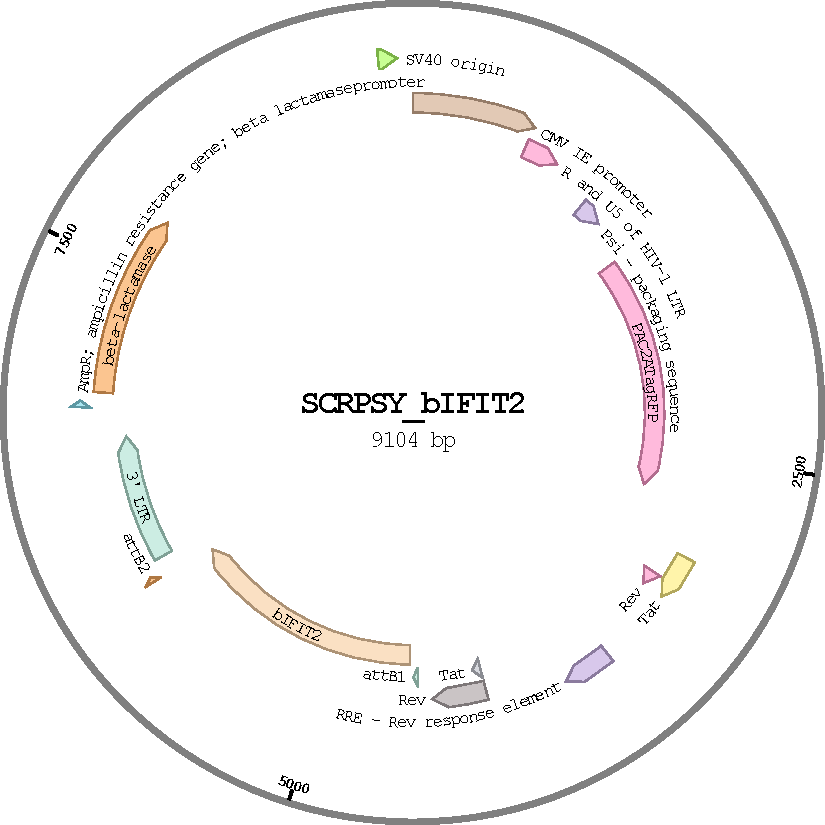
\includegraphics[width=0.6\linewidth]{05. Methods/Figs/01. scrpsy.pdf}
    \caption[SCRPSY Representative Map.]{\textbf{SCRPSY Representative Map.}}
    \label{fig:SCRPSY Representative Map}
\end{figure}

\begin{figure}
    \centering
    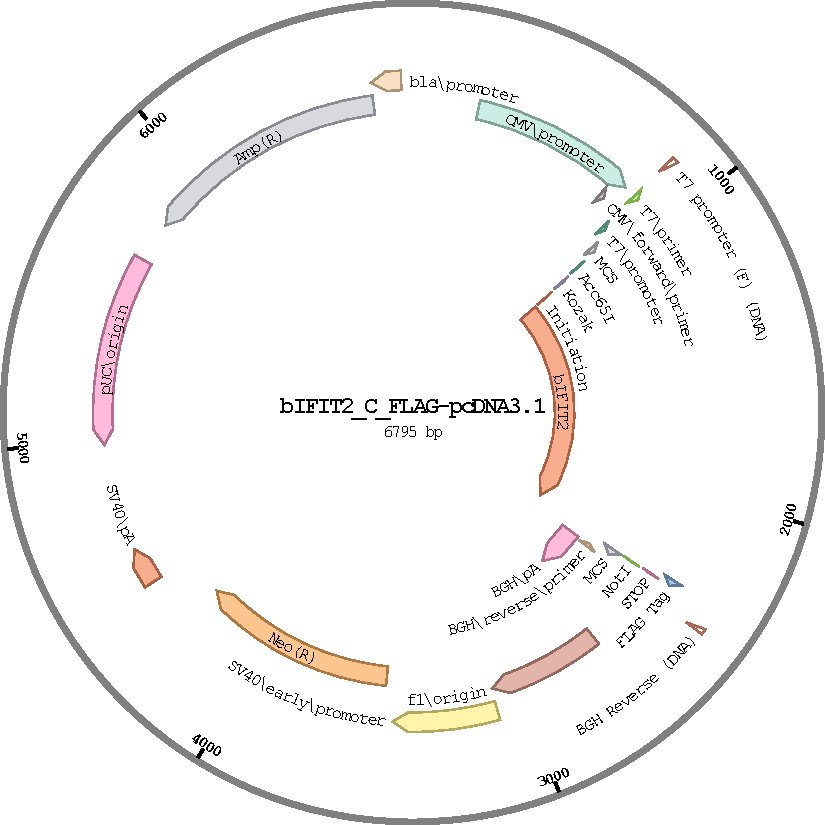
\includegraphics[width=0.6\linewidth]{05. Methods//Figs/02. pcDNA3.1.pdf}
    \caption[pcDNA3.1 Representative Map.]{\textbf{pcDNA3.1 Representative Map.}}
    \label{fig:pcDNA3.1 Representative Map}
\end{figure}

\subsection{Common Subcloning Methodologies} \label{subsec:Common Subcloning Methodologies}
\subsubsection[DNA Agarose Gel Electrophoresis and Extractions]{Analysis of DNA by Agarose Gel Electrophoresis and Gel Extractions} \label{Analysis of DNA by Agarose Gel Electrophoresis and Gel Extractions}
Linearised DNA was resolved and potentially isolated on 0.8\% agarose in tris-borate EDTA (TBE) buffer gel. 0.8\% agarose mixture was used as it provides resolution power greater than 10 kbp to 0.1 kbp. DNA visualisation was enabled by the addition of 15 µL ethidium bromide into 50 mL agarose TBE solution at circa 50°C prior to gel casting. DNA samples were mixed with 6X loading buffer (NEB) and loaded onto the gel. A DNA ladder was also electrophoresed in a separate well to allow size comparison. Samples were run at 80 V for 90 minutes. After the run, DNA bands were visualised using UV. Samples intended for gel purifications were excised from the gel using a clean scalpel and placed into clean 1.5 mL tubes.

\subsubsection{DNA Clean-Up After PCR or Gel Extraction} \label{DNA Clean-Up After PCR or Gel Extraction}
DNA clean-up was performed using the QiaQuick Gel Extraction Kit (Qiagen) following the manufacturer's protocol. In short, 3 volumes of buffer QC were added to either post-PCR DNA or to a gel slice (where 1 mg of gel was assumed to be equivalent to 1 µL). Samples were incubated at 50°C for 10 minutes, after which one sample volume of isopropanol was added to the samples. Samples were collected on a QIAquick spin column via centrifugation and washed with buffer PE twice. DNA was eluted to a 1.5 mL tube using centrifugation.

\subsubsection{DNA Ligation} \label{DNA Ligation}
20 µL total volume ligation reaction was prepared using DNA to be ligated, 2 µL T4 DNA ligase buffer (NEB), and 1 µL of T4 DNA ligase (NEB). Samples were incubated at 16°C for 72 hours.

\subsubsection[Transformation of \textit{E. Coli} and Bacterial Culture]{Transformation of Chemically Competent \textit{E. Coli} Cells and Bacterial Culture Amplification} \label{Transformation of Chemically Competent E.Coli Cells and Bacterial Culture Amplification}
2 µL of ligated samples or 1 µL of concentrated DNA were mixed with 25 µL \textit{E. coli} in 0.5 mL PCR tubes and placed in a PCR cycler. The samples were initially incubated at 4°C for 15 minutes, followed by a heat shock performed by incubating at 42°C for 45 seconds, followed by 2 minutes at 4°C. Afterwards, 75 µL of SOC solution was added, and the samples were left to incubate at 37°C for 60 minutes. Finally, 100 µL of the transformed bacterial culture was streaked on a room temperature agar plate containing ampicillin using a quadrant streaking method to ensure the establishment of a dilution gradient on the plate, allowing for single colony formation in the final quadrant. The plates were then incubated for 24 hours at 37°C. Finally, single colonies were picked, annotated, and amplified in LB broth containing 1 µL per mL of ampicillin for 24 hours at 37°C.

\subsubsection{DNA Purification and Sequencing} \label{DNA Purification and Sequencing}
Bacterial cultures from the final step of Section \ref{Transformation of Chemically Competent E.Coli Cells and Bacterial Culture Amplification} were pelleted by centrifugation at 4°C for 30 minutes at 4000 g. Depending on the size of the culture, plasmid DNA was purified using either the Miniprep or Midiprep kit (Qiagen; for 5 mL and 50 mL cultures, respectively) following the manufacturer's protocol and employing the alkaline lysis method. The final purified DNA was quality-assessed through restriction digestion followed by agarose gel electrophoresis (as described in Section \ref{Analysis of DNA by Agarose Gel Electrophoresis and Gel Extractions}). If successful, this process was followed by Sanger sequencing. The sequencing primers used for the ORFs of pcDNA3.1 plasmids were the forward T7 promoter primer and the reverse BGH primer.

\subsection{PCR for Cloning into pcDNA3.1} \label{subsec:PCR for Cloning into pcDNA3.1}
To create tagged bovine \textit{IFIT} ORFs and subclone them from the SCRPSY backbone into the pcDNA3.1 backbone, the following protocol was employed. Primers were designed based on the schematic in Figure \ref{fig:Schematic for PCR Primer Design}. The primers were 27-60 nucleotides in length, with melting temperatures established and utilised in the PCR protocol. PCR reaction mixtures with a final volume of 100 µL were prepared by combining 10 µL of 10X Pfu Buffer (Promega) with 100 ng of plasmid DNA, 4 µL of 5 nM dNTPs (NEB), 2 µL of Pfu DNA polymerase (Promega), 1 µL of 100 µM forward and reverse primers, and nuclease-free water. Samples were placed in a PCR thermocycler and incubated for 30 seconds at 98°C. This was followed by 30 cycles of 10 seconds at 98°C, 30 seconds at 58°C, and 90 seconds at 72°C. The final step was an incubation at 72°C for 2 minutes. To degrade the original plasmid material, samples were incubated with the DpnI restriction enzyme for 1 hour at 37°C. Afterwards, samples were cleaned as described in Section \ref{DNA Clean-Up After PCR or Gel Extraction}. The ORF amplicons had their ends digested by a sequential restriction digest with Acc65I (NEB) and NotI (NEB) restriction enzymes. This involved diluting samples with 10X 3.1 buffer into 1X, adding the restriction enzyme, incubating for 1 hour at 37°C, and heat-inactivating the enzyme at 65°C for 15 minutes. Digested amplicons were cleaned up as described in Section \ref{DNA Clean-Up After PCR or Gel Extraction}. The donor plasmid pcDNA3.1 was linearised using Acc65I and NotI restriction enzymes as described above, and gel-extracted as detailed in Section \ref{Analysis of DNA by Agarose Gel Electrophoresis and Gel Extractions} and Section \ref{DNA Clean-Up After PCR or Gel Extraction}. The linearised plasmid was dephosphorylated using Antarctic phosphatase (NEB). Amplicons and dephosphorylated plasmid were ligated in a 5:1 molar ratio, as described in Section \ref{DNA Ligation}.

\begin{figure}
    \centering
    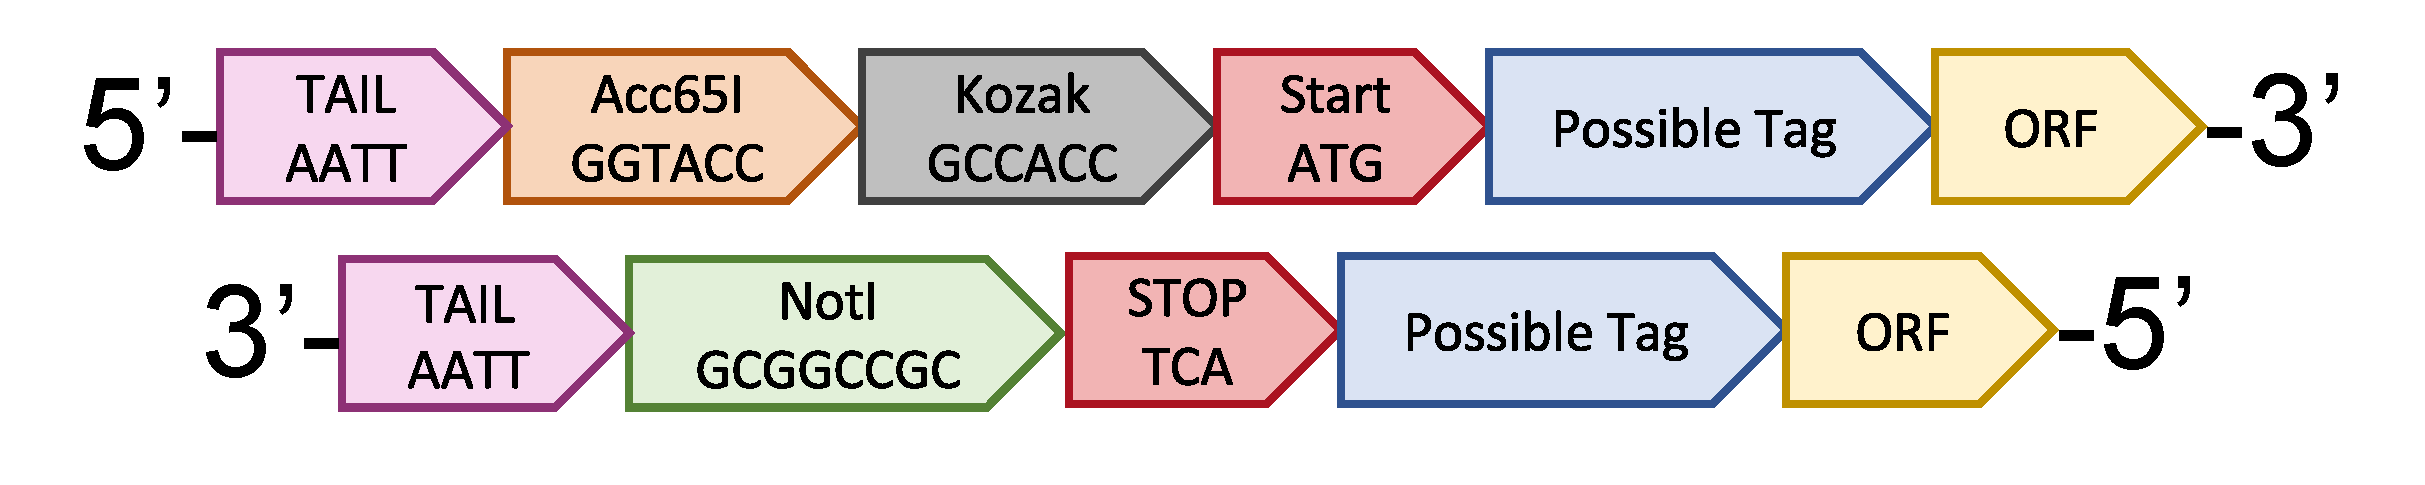
\includegraphics[width=1\linewidth]{05. Methods//Figs/03. cloning scheme.pdf}
    \caption[Schematic for PCR Primer Design.]{\textbf{Schematic for PCR Primer Design.}}
    \label{fig:Schematic for PCR Primer Design}
\end{figure}

\subsection{PCR for Point Mutant Generation} \label{subsec:PCR for Point Mutant Generation}
To create \textit{IFIT2} RNA-binding mutants, the following protocol was employed. The primers for hIFIT mutations were derived from the study by Tran \textit{et al.} \cite{Tran2020InfluenzaMRNAs} using inverse PCR methodology. bIFIT2 primers were based on the human ones. A protein model of the human IFIT2 complex, visualised in PyMol software \cite{SchrodingerTeam2023TheSystem}, had the amino acid residues 292 and 410 highlighted and compared to the residues on the corresponding place of predicted bovine IFIT2 structure. The effects of the mutations on the surfaces polarity was assayed \textit{in silico}. This established that the corresponding amino acid residues on the bovine IFIT2 that needed to be mutated were 289 and 402. The final primers can be seen in Table \ref{tab:Primers for Inverse PCR Mutagenesis table}, where the mutating nucleotides are shown using lowercase characters. PCR reaction mixtures with a final volume of 100 µL were prepared by combining 10 µL of 10X Pfu Buffer (Promega) with 100 ng of plasmid DNA, 4 µL of 5 nM dNTPs (NEB), 2 µL of Pfu DNA polymerase (Promega), 1 µL of 100 µM forward and reverse primers, and nuclease-free water. Samples were placed in a PCR thermocycler and incubated for 30 seconds at 98°C. This was followed by 30 cycles of 10 seconds at 98°C, 30 seconds at 58°C, and 200 seconds at 72°C. The final step was incubation at 72°C for 2 minutes. To degrade the original plasmid material, samples were incubated with DpnI restriction enzyme for 1 hour at 37°C. Afterwards, samples were cleaned as described in Section \ref{DNA Clean-Up After PCR or Gel Extraction} and eluted in 20 µL of nuclease-free water. DNA was phosphorylated by adding 2 µL of 10X ligase buffer and 1 µL of T4 Polynucleotide Kinase (NEB), incubating the samples for 30 minutes at 37°C. The enzyme was then inactivated by incubation at 65°C for 20 minutes. Finally, samples were ligated by the addition of 1 µL of T4 DNA ligase, followed by incubation at 16°C for 72 hours.

\begin{table}
\centering
\begin{tabular}{ll}
\toprule
\textbf{Primer Name}   & \textbf{Sequence 5$^{\prime}$-3$^{\prime}$}    \\ \midrule
hIFIT2   R292E forward & GTGCTGCTATgagGCAAAAGTCTTC  \\ 
hIFIT2 R292E reverse   & CCAATTTGGCAATGCAGG         \\ 
hIFIT2   K410E forward & GGAGAAAGAAgagATGAAAGACAAAC \\ 
hIFIT2 K410E reverse   & CTTGATTTCTGGTTTATTTTTACAC  \\ 
bIFIT2   R287E forward & GTGCTGCTATgagGCCAAAGTCCT   \\ 
bIFIT2 R287E reverse   & CCAATATGGCAATGCAGG         \\ 
bIFIT2   K401E forward & GAAGGAGAAgaaATGAAAAACAAAC  \\ 
bIFIT2 K401E reverse   & CTTTGATCCCTGGTTTAT         \\ \bottomrule
\end{tabular}
\caption[Primers for Inverse PCR Mutagenesis.]{\textbf{Primers for Inverse PCR Mutagenesis.}}
\label{tab:Primers for Inverse PCR Mutagenesis table}
\end{table}

\section{Confocal Microscopy} \label{sec:Confocal Microscopy}
Cells grown on a 13 mm diameter glass coverslip (Agar Scientific), were washed with PBS and fixed by incubating in 4\% paraformaldehyde (Sigma-Aldrich) at room temperature for 15 minutes at the endpoint of the experiments. Subsequently, samples were permeabilised by incubating in a 0.2\% Triton X-100/PBS solution for 5 minutes. Residual Triton was removed by PBS washes, followed by blocking the coverslips using 1\% bovine serum albumin (BSA; Sigma-Aldrich) in PBS for at least 30 minutes. Samples were then incubated overnight with the primary antibody in a 1\% BSA in PBS solution, diluted as specified in Table \ref{tab:Antibodies for Confocal Microscopy}. Afterwards, they were washed again with PBS and incubated for an hour at room temperature with secondary antibodies diluted in a 1\% BSA in PBS solution, as specified in Table \ref{tab:Antibodies for Confocal Microscopy}. The nuclei of the cells were stained with 4,6-diamidino-2-phenylindole (DAPI; Abcam), diluted 1:20,000 in water. After a 10-minute incubation, residual DAPI was washed away with water, followed by an additional wash with PBS. Stained slides were mounted on glass slides using Vectashield (Vector Labs). Confocal images were acquired on Leica TCS SP5 and Zeiss LMS700 confocal microscopes using 405 nm, 488 nm, and 568 nm laser lines with a 63X oil immersion objective. Laser lines were operated sequentially to prevent bleed-through, and image quality was enhanced by frame averaging. The pinhole was set to 1 airy unit. Maximal laser line gains were established per experiment using secondary antibody-only controls, while minimal gains were established using the maximum intensity of sample slides, allowing for a maximum range of signal acquisition. Images were scaled using bilinear interpolation. Image analysis, including annotation and calculation of inclusion body diameter and area, along with the assessment of colocalisation, was conducted in QuPath software \cite{Bankhead2017QuPath:Analysis}. The final figures were constructed in Fiji software \cite{Schindelin2012Fiji:Analysis} using the QuickFigures plugin \cite{Mazo2021QuickFigures:Figures}.

\begin{table}
\centering
\begin{tabular}{llll}
\toprule
\textbf{Antibody Target} & \textbf{Host Species} & \textbf{Provider} & \textbf{Working Dilution} \\ \midrule
RSV N       & Mouse  & Taylor \textit{et al.}, 1992 \cite{Taylor1992ProtectiveAntibodies.}             & 1:400   \\
RSV P       & Mouse  & Taylor \textit{et al.}, 1992 \cite{Taylor1992ProtectiveAntibodies.}              & 1:400   \\
RSV   M2/1  & Mouse  & Taylor \textit{et al.}, 1992 \cite{Taylor1992ProtectiveAntibodies.}              & 1:400   \\
IFIT1       & Rabbit & Invitrogen        & 1:200   \\
IFIT2   (A) & Rabbit & Proteintech       & 1:200   \\
IFIT2 (B)   & Rabbit & Novus Biologicals & 1:200   \\
IFIT3       & Rabbit & Proteintech       & 1:200   \\
IFIT5       & Rabbit & Invitrogen              & 1:200   \\
FLAG        & Rabbit & Invitrogen              & 1:200   \\
Rabbit Igg  & Goat   & Invitrogen              & 1:10000 \\
Mouse   Igg & Goat   & Invitrogen              & 1:10000 \\ \bottomrule
\end{tabular}
\caption[Antibodies for Confocal Microscopy.]{\textbf{Antibodies for Confocal Microscopy.}}
\label{tab:Antibodies for Confocal Microscopy}
\end{table}

\section{Statistical Analysis} \label{sec:Statistical Analysis}
Statistical analysis was conducted using the R programming language \cite{RCoreTeam2022R:Computing} within the RStudio environment \cite{RStudioTeam2022RStudio:RStudio}. URL http://rpubs.com/ogosimiso/995988 hosts the entire statistical analysis pipeline. Initially, data were visually assessed using boxplots and Q-Q plots. Boxplots provided a rough evaluation of normality, while Q-Q plots were employed for a preliminary assessment of the equality of variances. The normality of distribution was further tested using the Shapiro-Wilk normality test, performed individually for each condition and for the entire dataset. The equality of variance was evaluated through the Bartlett test of homogeneity of variances for normally distributed samples and Levene's Test for Homogeneity of Variance (car package for R \cite{Fox2019AnRegression}) for non-normally distributed samples. To derive final significance values, various statistical tests were applied based on the number of comparisons and the distribution and equality of variances. For a pair of samples with normal distribution and equal variance, a two-sample t-test was conducted. Multiple comparisons of normally distributed data with equal variance were performed using analysis of variance (ANOVA) combined with Tukey's multiple comparisons of means. For a pair of samples with non-normal distribution but equal variance, a two-sample t-test was employed. Multiple comparisons of non-normally distributed data with equal variance were subjected to the Kruskal-Wallis rank sum test (dunn.test R package \cite{Dinno2017Dunn.test:Sums}). For a single comparison of data with a normal distribution but non-equal variance, a Welch Two-Sample t-test was executed. Multiple comparisons of data with normal distribution but non-equal variance were subjected to one-way analysis of means (not assuming equal variances), combined with the Games-Howell test (rstatix R package \cite{Kassambara2022Rstatix:Tests}).

%Words in text: 3897
%Words in headers: 117
%Words outside text (captions, etc.): 61
%total = 4075
